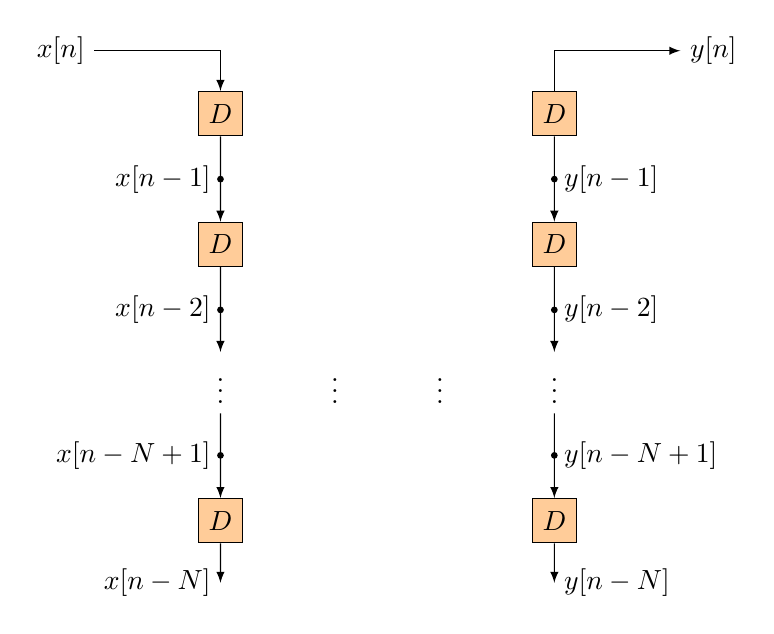
\begin{tikzpicture}
[
	scale=0.8,
	delay/.style={draw=black, fill=orange!40, minimum width=1.6em, minimum height=1.6em},
	adder/.style={circle, draw=black, fill=pink!40, minimum width=1.2em, minimum height=1.2em, inner sep=0},	
	br/.style={circle, draw=black, fill=black, minimum width=0.2em, minimum height=0.2em, inner sep=0},		
]

      \matrix (m) [row sep=5mm, column sep=10mm]{
      \node [delay] (m00) {$D$}; &  &  & \node [delay] (m03) {$D$}; \\
      \node [br] (m10) {}; &  & & \node [br] (m13) {};\\
      \node [delay] (m20) {$D$}; &  & & \node [delay] (m23) {$D$}; \\
      \node [br] (m30) {}; &   & & \node [br] (m33) {};\\
      \node [] (m40) {$\vdots$}; & \node [] (m41) {$\vdots$};   & \node [] (m42) {$\vdots$};  & \node [] (m43) {$\vdots$}; \\
      \node [br] (m50) {}; &  &    & \node [br] (m53) {};\\
      \node [delay] (m60) {$D$}; & &  & \node [delay] (m63) {$D$}; \\
      \coordinate (m70) {}; &   &   & \coordinate (m73) {};\\
      };


%
%
  

      \foreach \i/\j in {0/2, 2/4, 4/6}
    {
		\draw[-latex] (m\i 0) -- (m\j 0);
		\draw[-latex] (m\i 3) -- (m\j 3);		
    }


      \foreach \i/\j in {6/7}
    {
		\draw[-latex] (m\i 0) -- (m\j 0);
		\draw[-latex] (m\i 3) -- (m\j 3);		
    }

%     \draw[-latex] (m00) -- node[midway, above] {$b_0$} (m01);
%     \draw[-latex] (m02) -- node[midway, above] {$1/a_0$} (m03);
% 
     \draw (m10) node[anchor=east] {$x[n-1]$};
     \draw (m13) node[anchor=west] {$y[n-1]$};

    \draw (m30) node[anchor=east] {$x[n-2]$} ;
    \draw (m33)  node[anchor=west] {$y[n-2]$};

    \draw (m50) node[anchor=east] {$x[n-N + 1]$};
    \draw (m53)  node[anchor=west] {$y[n-N + 1]$};

    \draw (m70) node[anchor=east] {$x[n-N]$} ;
    \draw (m73)  node[anchor=west] {$y[n-N]$};

    \draw[latex-] (m00) |- ++(-2, 1) node[anchor=east] {$x[n]$};
    \draw[-latex] (m03) |- ++(2, 1) node[anchor=west] {$y[n]$};

    %\pause
    %\draw[-latex] (m01) -- node[midway, above] {$w[n]$} (m02);
\end{tikzpicture}